    \documentclass[15pt]{article}
\marginparwidth 0.5in 
\oddsidemargin 0.25in 
\evensidemargin 0.25in 
\marginparsep 0.25in
\topmargin 0.25in 
\textwidth 6in 
\textheight 8 in

\usepackage{graphicx}
\frenchspacing

\usepackage{amsmath}
\begin{document}
\vskip 1cm

\begin{figure}[htp]
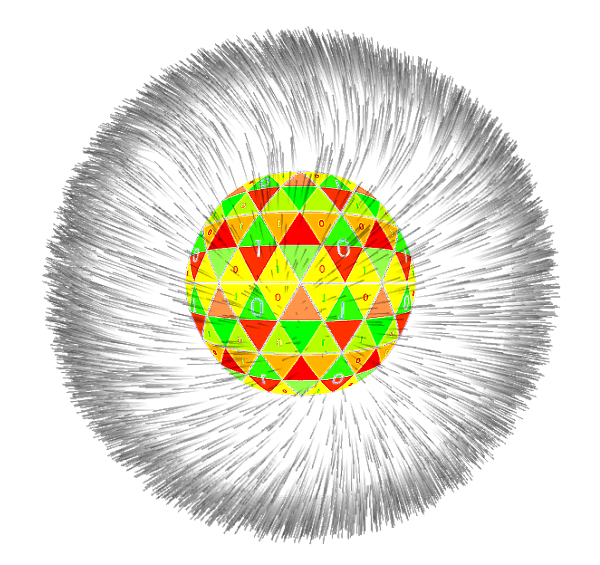
\includegraphics[scale=0.70]{./img/artee-1.png}
\caption{data-nodes arround a context domain space (mind's eye)}

\end{figure}


\title{\textbf{ACTIVE-MEMORY}}
\author{Hagen Geissler / santex\\
		C3D2}
\date{2012}


\maketitle


$\rightarrow$ \textbf{https://github.com/santex/active-memory-paper}
%-----------------------------------------------------------


\begin{center}


{\bf Short Description} \\[0.4cm]

\textbf{Procreating data}, under fitness consideration,
      in form of \textbf{semantic} micro-structures 
      within a conceptional domain.
      controlled by a human users request.
\vskip0.5cm


\begin{flushleft}


The projects goal is to establish a way to compound information quality  , quantity in a genetic fashion.

\vskip0.5cm

To organise knowledge like a biological organism. within a data population.

on data-nodes which are organisation,
in a context domain space.
Goal is to facilitate procreation in a genetic fashion. in essence to make better information from information.

Desired result of all efforts is to make better data from data by default.

It also has very interesting organisational properties,
each structure is bound on a concept or more.

Side effect of the genetic fitness evaluation
is that all root nodes and end nodes are known upfront reducing
query distance as each end-node is same distance.
It enables us to work kind of parallel.

\end{flushleft}




{\small New Terms } \\[0.1cm]
\textbf
{micro-structure}\\  
a micro-structure is a abstract entity describing 
\textbf{any concept}\\
the information is obtained via \textbf{WORD-NET}\\
\vskip0.4cm
\textbf
{key-stone}\\  
a key-stone is the root of a micro-structure 
\vskip0.4cm
\textbf
{example:}\\  
a micro-structure with the key-stone existence
\vskip0.2cm

\end{center}


          \begin{verbatim}
          <existence>
          - Cosmos
          - Unit
          - Universe
          - Physical_entity
          - Object
          - Physical_object
          - Nature
          - Macrocosm
          - Natural_order
          - World
          - Whole
          - Natural_object
          - Closed_universe
          - Existence
          - Creation
          - Entity
          \end{verbatim}


\vskip 1cm


\subsection{combining to a complex entity}
\begin{flushleft}	
\begin{figure}[htp]
\centering
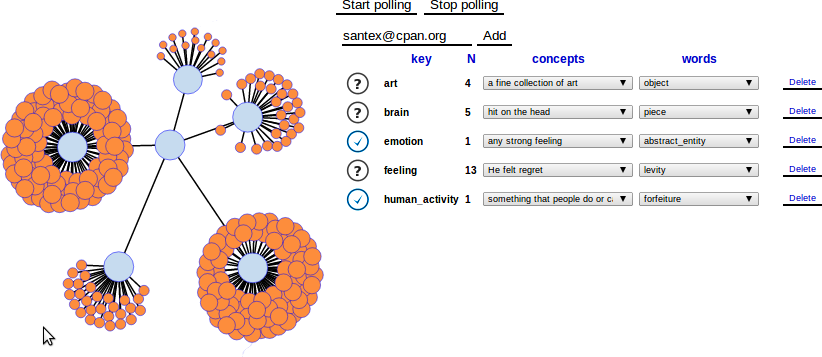
\includegraphics[scale=0.55]{./img/micro-structure-creation-implement.png}
\caption{making micro-structures}
\label{}
\end{figure}
\end{flushleft}
\begin{tabular}{lll}
	concept art & 4 sub-concepts & 27 key-words\\
	concept brain & 5 sub-concepts &  16 key-words\\
	concept emotion & 1 sub-concept &  28 key-words\\
	concept feeling & 13 sub-concepts &  76 key-words\\
	concept human-activity & 1 sub-concepts &  83 key-words\\

\end{tabular}
\vskip 1cm
	The core node is my user-name
\begin{flushleft}	
\begin{figure}[htp]
\centering
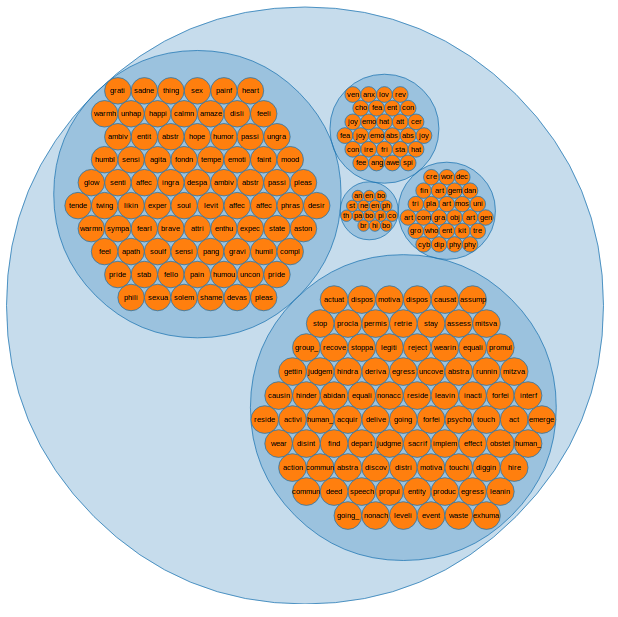
\includegraphics[scale=0.80]{./img/circle.png}
\caption{pack of concepts}
\end{figure}
\end{flushleft}
\vskip 5cm
\subsection{micro-structure properties}


\begin{itemize}
\item a micro-structure lives as a perl module (\$micro new existence)
\item most human concepts available
\item combine modular
\item access via terminal
\item micro-structure have access to the data-plug-in's (wiki, google, torrent)
\item the micro-structure is used as permanent query to scan for data.
\end{itemize}


\subsection{active-memory plug-ins}

\begin{itemize}
\item plug-ins are like feeds to just compatible to micro-structure's
\item currently in use wiki plug-in (google planed)
 

\end{itemize}



\vskip 2cm


\section{Fitness}  
  
Variables $\rightarrow$   

\begin{itemize}
\item C-total Word-net concept sum
\item C-established used concept sum
\item generation 
\item spawning links sum \textbf{in individual}
\item tag-number sum \textbf{in individual}
\item tag-ratios across total data population in micro-structure
\item tag-density across total data population in micro-structure
\item media items ratio \textbf{(links/amount media items)} (ogg, image, pdf)
\item special items ratio \textbf{(links/amount special items)} (category, list)
\item amount non linking/spawning individuals/
\end{itemize}

\vskip 0.4cm

\section{continuum of concepts within a micro-structure}  
  
\begin{itemize}
\item $\rightarrow$ \textbf{object}
\item natural object|physical object|celestial body|heavenly body
\item planet
\item outer planet
\item jovian planet
\item superior planet
\item major planet
\item gas giant
\item jupiter
\item Iapetus
\item moon
\item satellite
\item heavenly body|celestial body|physical object|natural object 
\item $\rightarrow$ \textbf{object};
\end{itemize}   


\section{dealing with sub concepts of a higher order}

      \begin{verbatim}

my personal implementation please note there is a chance that things are broken at the time you looking on it.
try bit later or send a mail

http://algoservice.com:5984/wikilist/_design/base/micro.html
bzw:
http://algoservice.com:5984/wikilist/_design/base/micro-wiki.html
  
this is a representation of ca 200.000 result-nodes across a large number of (category's / micro-structure requests)

the page still changes very frequently but normally it will provide a on the fly semantic within the end nodes 
by next-neighbor approximation as demonstrated in the right panel on the page 

wait until web socket is connected (http://algoservice.com:5984/wikilist/_design/base/micro.html) then search biology 


next neighbor's of "biology" and the  density of crossovers 

(biology) = 4382  Article/end-nodes in population
(biology, anatomy) = 161 Article/end-nodes in population

next neighbour's
biology: 4382
anatomy: 161
genetics: 155
zoology: 123
ecology: 86
botany: 63
chemistry: 63
medicine: 48
medical: 47
unit: 42
genus: 41
wine: 40
animal: 39
mollusc: 39
evolution: 37
mycology: 37
journal: 36
epidemiology: 35


this way we are able to create a ontology over huge amount of data,
as we interpolate over knowledge.
its similar to a tetra-eder network.
or a Voronoi_diagram.

http://quantup.com/lib/3d/examples/voroboids/voroboids.html
http://upload.wikimedia.org/wikipedia/commons/8/89/2Ddim-L2norm-10site.png


the group,
of most dense nodes (swanning & categories),
build the point of convergence, like in the Voronoi_diagram.

Please note that these 200.000 nodes come from my space micros-structure , 
its de-central 

normally,
you would have your own structure and end-nodes,
across what ever concepts you fancy.


    
$. sudo micro new hacker

returns 
organism

               .--'"""""--.>_
            .-'  o\\b.\o._o.`-.                 
         .-'.- )  \d888888888888b.
        /.'   b  Y8888888888888888b.
      .-'. 8888888888888888888888888b
     / o888 Y Y8888888888888888888888b
     / d888P/ /| Y"Y8888888888888888888b
   J d8888/| Y .o._. "Y8888888888888Y" \
   |d Y888b|obd88888bo. """Y88888Y' .od8
   Fdd 8888888888888888888bo._'|| d88888|
   Fd d 88\ Y8888Y "Y888888888b, d888888P
   d-b 8888b Y88P'     """""Y888b8888P"|
  J  8\88888888P    `m.        """""   |
  || `8888888P'       "Ymm._          _J
  |\\  Y8888P  '     .mmm.YM)     .mMF"'
  | \\  Y888J     ' < (@)>.- `   /MFm. |
  J   \  `YY           ""'   ::  MM @)>F
   L  /)  88                  :  |  ""\|
   | ( (   Yb .            '  .  |     L
   \   bo  8b    .            .  J     |        The word hacker
    \      "' .      .    .    .  L   F         has 4 concept's
     o._.:.    .        .  \mm,__J/  /          we need to find out the which one
     Y8::'|.            /     `Y8P  J           to use for our new,
     `|'  J:   . .     '   .  .   | F           micro-structure,
      |    L          ' .    _:    |            
      |    `:        . .:oood8bdb. |            
      F     `:.          "-._   `" F            



(1): someone who plays golf poorly      
(2): a programmer who breaks into computer systems 
	     in order to steal or change or destroy information as a form of cyber-terrorism
	     
(3): a programmer for whom computing is its own reward; 
	 may enjoy the challenge of breaking into other computers 
	 but does no harm true hackers subscribe to a code of ethics
	 and look down upon crackers
	 
(4): one who works hard at boring tasks
                                                
  Type: the number you choose 1..4
 #my choice of sub-concept
$. 3
returns

hacker
programmer
computer_programmer
coder
software_engineer
engineer
applied_scientist
technologist
person
individual
someone
somebody
mortal
soul
organism
being
living_thing
animate_thing
whole
unit
object
physical_object
physical_entity
entity
causal_agent
cause
causal_agency
physical_entity
entity
computer_user
person
individual
someone
somebody
mortal
soul
organism
being
living_thing
animate_thing
whole
unit
object
physical_object
physical_entity
entity
causal_agent
cause
causal_agency
physical_entity
entity
hacker
programmer
computer_programmer
coder
software_engineer


\end{verbatim}


\vskip 1cm




\section{Project code structure}

\begin{itemize}
\item $\rightarrow$ \textbf{perl module}
\item $\rightarrow$ \textbf{memcache}
\item $\rightarrow$ \textbf{couchdb}
\item $\rightarrow$ \textbf{wordnet}
\end{itemize}   



\section{experimental Implementation}

\begin{itemize}
\item $\rightarrow$ \textbf{ui: http://www.quantup.com}
\item $\rightarrow$ \textbf{data-base: http://algoservice.com:5984/wikilist/}
\item $\rightarrow$ \textbf{git: https://github.com/santex/active-memory}

\end{itemize}   

\section{Network}
    
   \begin{tabular}{cc}
    Data in disorganised data network         &    The same network as micro-structure\\
    
    \end{tabular}




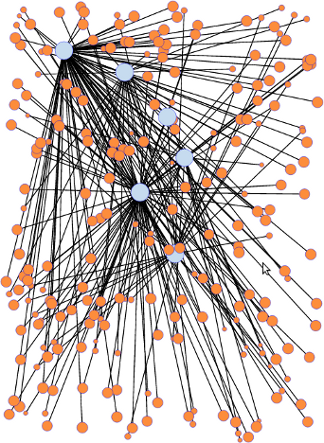
\includegraphics[scale=0.5]{img/normal-knowledge.png}
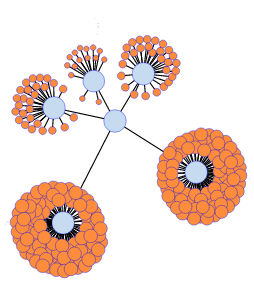
\includegraphics[scale=0.9]{img/micro-structure.png}


\vskip 0.4cm

    \begin{tabular}{cc}
    Data in disorganised data network           &|    The same network as micro-structure\\
    \\

    \end{tabular}

\section{A sample}

  \begin{verbatim}

~$ micro hacker
computer_user

~$ micro hacker
programmer

now use > $ micro hacker 20
animate_thing
programmer
object
coder
computer_programmer
physical_object
living_thing
entity
software_engineer
physical_entity
engineer
cause
individual
applied_scientist
being
hacker
somebody
technologist
causal_agent
whole



  \end{verbatim}


\vskip 1cm


\section{A sample with data}


  \begin{verbatim}


   $ micro new constallation;
   $ micro constallation 103;
   
   
   
    andromeda
    antlia
    apus
    aquarius
    aquila
    ara
    argo
    aries
    auriga
    bootes
    caelum
    cancer
    canis_major
    canis_minor
    capricorn
    capricornus
    carina
    cassiopeia
    centaur
    centaurus
    cepheus
    cetus
    chamaeleon
    chameleon
    charioteer
    circinus
    columba
    coma_berenices
    constellation
    corona_borealis
    corvus
    crane
    crater
    crow
    crux
    crux_australis
    cygnus
    delphinus
    dorado
    dove
    draco
    dragon
    entity
    eridanus
    fornax
    gemini
    great_bear
    great_dog
    grus
    hercules
    hunter
    hydra
    hydrus
    indus
    leo
    lepus
    libra
    little_bear
    little_dog
    lupus
    lyra
    mensa
    microscopium
    musca
    natural_object
    norma
    object
    octans
    ophiuchus
    orion
    pavo
    pegasus
    perseus
    phoenix
    physical_entity
    physical_object
    pictor
    pisces
    puppis
    pyxis
    reticulum
    sagitta
    sagittarius
    scorpio
    scorpius
    sculptor
    serpens
    snake
    southern_cross
    southern_triangle
    taurus
    telescopium
    triangle
    triangulum
    triangulum_australe
    tucana
    unit
    ursa_major
    ursa_minor
    vela
    virgo
    volans
    vulpecula
\end{verbatim}
\vskip 1cm

get data this shell script only to balance load regular command 


(micro-wiki virgo)
.............................................................
\vskip 1cm

\begin{verbatim}
#!/bin/bash
IFS_BAK=$IFS;
IFS=$'\n';
array=( $(micro constallation 105) );
n=0;
for item in ${array[@]}
do
var=$(ps aux | grep -c perl);
if  [ 80 -lt $var ]; 
then 
  echo $n;
  sleep 10;
else
  micro-wiki $item &
fi
  let n+=1
done;
echo $n;
IFS=$IFS_BAK;
\end{verbatim}

\vskip 1cm

downloading\\
.............................................................\\

    
\begin{flushleft}
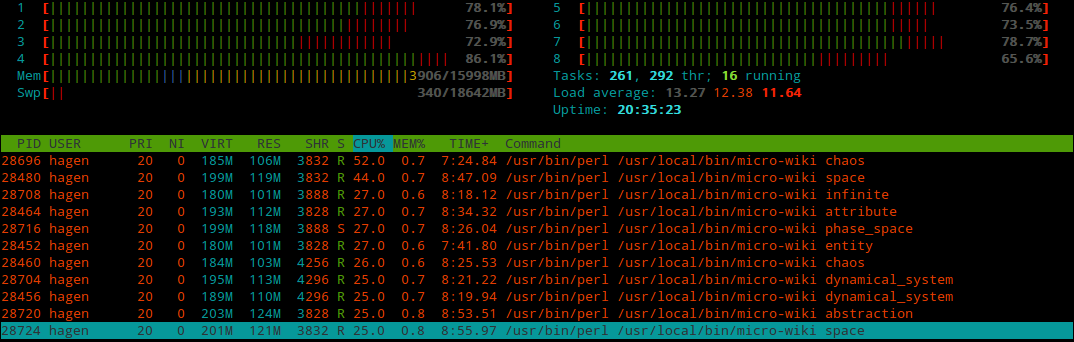
\includegraphics
[scale=0.43]{img/plugin.png}
\end{flushleft}
\vskip 1cm

sample out images (actually the image results are times 5)\\
.............................................................\\

    
\begin{flushleft}
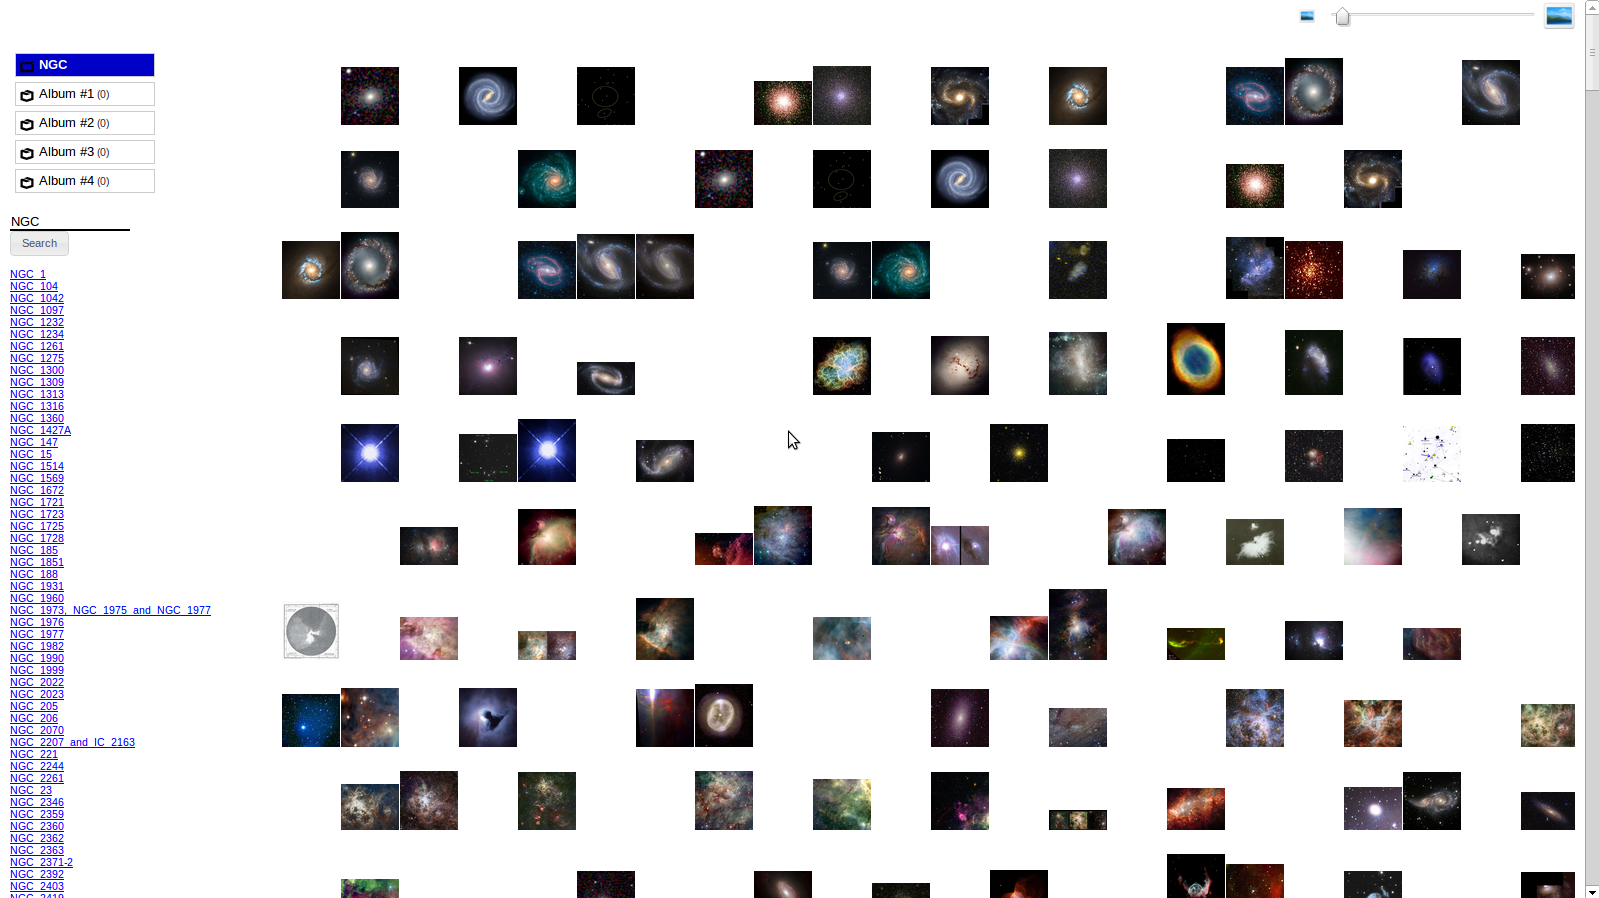
\includegraphics
[scale=0.29]{img/result-images.png}
\end{flushleft}
\vskip 5cm

\end{document}
  